% !TeX root = ../apuntes-ea.tex

\chapter{Anillos (y cuerpos)}

En este capítulo se extiende lo que sabemos de teoría de grupos a las nuevas estructuras algebraicas que introducimos que son los anillos y los cuerpos.

\section{Definición y propiedades básicas}

\begin{dfn}[Anillo]
	Un anillo es una terna $(A, +, \cdot)$ donde $+: A \times A \to A$ es una operación a la que llamamos suma, $\cdot: A \times A \to A$ es otra operación a la que llamamos producto y se verifican las siguientes propiedades
	\begin{enumerate}
		\item El par $(A, +)$ es un grupo abeliano
		\item El producto $\cdot$ es asociativo
		\item Se cumplen las propiedades distributivas:
		\begin{align}
			\forall a, b , c \in A,\ a\cdot (b + c) = a\cdot b + a \cdot c \\
			\forall a, b , c \in A,\ (a + b) \cdot c = a\cdot c + b \cdot c
		\end{align}
	\end{enumerate}
\end{dfn}

Con la operación $+$ tenemos las siguientes propiedades
\begin{enumerate}
	\item Asociatividad: $(a+b)+c = a+(b+c)$
	\item Elemento neutro aditivo: $\exists! \0 \in A \mid \0+a = a$
	\item Elemento inverso aditivo: $\forall a \in A, \exists -a \in A \mid a + (-a) = \0$
	\item Conmutatividad aditiva: $\forall a, b \in A,\ a+b = b+a$
\end{enumerate}

Con la operación $\cdot$ tenemos las siguientes propiedades
\begin{enumerate}
	\item Asociatividad: $a\cdot (b \cdot c) = (a \cdot b) \cdot c$
	\item No siempre existe el neutro multiplicativo: $\1 \in A \mid a\cdot 1 = 1 \cdot a = a$
	\item No siempre el producto es conmutativo.
	\item No siempre existe inverso multiplicativo: $\inv{a} \mid a\cdot \inv{a} = \1$
	\item No siembre se da la conmutatividad multiplicativa: $a \cdot b = b\cdot a$
\end{enumerate}

\begin{pro}
	$\forall a \in A,\ a\cdot \0 = \0$
\end{pro}

\begin{proof}
	$a \cdot \0 = a \cdot(\0 + \0) = a\cdot \0 + a\cdot \0 \implies \0 = a\cdot \0$
\end{proof}

\begin{dfn}[Anillo con unidad o anillo unitario]
	Sea $(A, +, \cdot)$ un anillo. Decimos que es un anillo con unidad o un \underline{anillo unitario} si tiene elemento neutro multiplicativo, es decir, si $\exists \1 \in A \mid \forall a \in A, \1 a = a \1 = a$.
\end{dfn}

\begin{pro}
	El neutro multiplicativo o unidad, $\1$, si existe, es único.
\end{pro}


\begin{dfn}[Anillo conmutativo]
	Sea $(A, +, \cdot)$ un anillo. $A$ es un anillo conmutativo $\iff \forall a, b \in A,\ a\cdot b = b \cdot a$. Es decir, un anillo es conmutativo $\iff$ el producto también es conmutativo.
\end{dfn}

\begin{pro}
	Sea $(A, +, \cdot)$ un anillo con más de un elemento ($|A| > 1$). Entonces $\0 \neq \1$ (el neutro aditivo es distinto del neutro multiplicativo).
\end{pro}

\begin{proof}
	Por contradicción. Sea $a \neq \0 \in A$ y $\0 = \1$. Entonces $a = a\cdot \1 = a\cdot 0 = 0 \implies a = \0$ contradicción.
\end{proof}

Para acabar veremos ejemplos de los 4 posibles casos que se pueden dar con las dos definiciones anteriores:

\begin{ej}[Anillo conmutativo con unidad]
	El anillo $(\Z, +, \cdot)$ es un anillo con unidad y la unidad es $\1 = 1$.
\end{ej}

\begin{ej}[Anillo conmutativo sin unidad]
	El anillo $(2\Z, +, \cdot)$ no tiene unidad ya que $\nexists \1 \in 2\Z \mid \forall a \in 2\Z,\ a\1 = \1a = a$.
\end{ej}

\begin{ej}[Anillo no conmutativo con unidad]
	Las matrices cuadradas $2\times 2$ con coeficientes reales: $(M_{2\times 2}(\R), +, \cdot)$ es un anillo con unidad (el neutro multiplicativo es $\1 = I$) pero no es conmutativo.
\end{ej}

\begin{ej}[Anillo no conmutativo sin unidad]
	Las matrices cuadradas $2\times 2$ con coeficientes en $2\Z$ es un anillo no conmutativo y además no tiene unidad.
\end{ej}

El ejemplo menos enrevesado es el primero. También son ejemplos de anillos conmutativos con unidad los conjuntos habituales $\mathbb{Q}, \R, \mathbb{C}$ y los conjuntos de clases $\Z/p\Z$ con $p$ primo (en todos ellos el neutro multiplicativo es lo que te esperas que sea el neutro multiplicativo). Además todos ellos cumplen que el conjunto con el producto es un grupo. Pues como es tan común esta cosa le damos nombre:

\begin{dfn}[Cuerpo (alternativa)]
	Sea $(A, +, \cdot)$ un anillo conmutativo con unidad. Diremos que $A$ es un cuerpo si $A\setminus \{\0\}$ es cerrado por la segunda operación (el \textit{producto}).
\end{dfn}

Es decir, que $(A\setminus\{\0\}, \cdot)$ es un grupo. Digo definición alternativa porque la definición que ha dado Orlando es ligeramente diferente (hay que esperar media página para conocerla pero es la \autoref{dfn:cuerporlando}).

\begin{ej}
	\item $\Z/p\Z$ con $p$ primo es un cuerpo
	\item $\Z$ o $\Z/6\Z$ no son cuerpos
	\item $\Q$ es un cuerpo (es el primero que sale al ir añadiendo números a los naturales)
	\item $\R$ y $\mathbb{C}$ también son cuerpos
	\item Las matrices $2 \times 2$ invertibles que antes veíamos como un grupo solo con el producto también son un cuerpo si les añadimos la suma: $(GL_2(\R), +, \cdot)$ es un cuerpo.
\end{ej}

Antes de seguir, siempre vamos a hablar de anillos con unidad o \textbf{anillos unitarios}, aunque alguna vez se me olvide ponerlo.

\subsection{Extensiones de anillos}
\begin{dfn}[Extensión de anillos]
	Sea $(A, +, \cdot)$ un anillo. Definimos la extensión
	\begin{align}
		A[m] = \{a+bm \mid a, b \in A\}
	\end{align}
\end{dfn}

\begin{ej}La extensión de los reales con $i = \sqrt{-1}$ son los complejos:
	\begin{align*}
		\R[\sqrt{-1}] = \{a+bi \mid a,b \in \R\} = \mathbb{C}
	\end{align*}
\end{ej}

\subsection{Unidades en anillos}

Además, para pulir lo de que no siempre existe inverso multiplicativo daremos la definición de Grupo de unidades en el contexto de anillos que da sentido al \autoref{ej:grupounidades} que hemos estado utilizando. Ojo: aquí unidades no se refiere a varios elementos neutros multiplicativos como uno podría pensar.

\begin{dfn}[Unidades en anillos]
	Dado $(A, +, \cdot)$ anillo. El grupo de unidades es
	\begin{align}
		\uds{A} = (\{a \in A \mid \exists \inv{a} \in A,\ a\cdot \inv{a} = \1\}, \cdot)
	\end{align}
	Los elementos del grupo de unidades se llaman \textbf{elementos invertibles}.
\end{dfn}

Para que este grupo quede bien definido estaría bien que $\inv{a}$ fuera único.

\begin{pro}
	El inverso multiplicativo es único.
\end{pro}

\begin{proof}
	Sea $a \in A$. Supongamos $a', a'' \in A$ son ambos inversos multiplicativos de $a$:
	\begin{align*}
		aa' = \1 \land aa'' = \1\implies \begin{cases}
		a''(aa') = a'' \\
		(a''a)a' = a''
		\end{cases}\implies a' = a''
	\end{align*}
\end{proof}

\begin{pro}
	Sea $-\1$ el inverso aditivo del neutro multiplicativo $\1$. Entonces $\forall a \in A$ el inverso aditivo es $-a = -\1 \cdot a$ y se tiene $-\1\cdot a + a = 0$.
\end{pro}

\begin{pro}
	Sea $A$ un anillo. El neutro aditivo $\0$ verifica $\0 \not\in \uds{A}$
\end{pro}

\begin{pro}[Propiedad cancelativa]
	Sea $a \in \uds{A}$. Entonces $\forall b,c$ se tiene $b, c \in A \implies a\cdot b = a\cdot c \implies b = c$
\end{pro}

\begin{pro}
	$a \in \uds{A} \iff \gen{a} = A$
\end{pro}

\begin{proof}$ $\newline
	\begin{enumerate}
		\item $(\implies)\qquad a \in \uds{A} \implies \exists \inv{a} \implies \gen{a} = A\cdot a = \{\alpha a \mid \alpha \in A\}$. Si $a \in \uds{A} \implies \exists \inv{a} \implies \inv{a}a = \1 \in \gen{a} \iff \gen{a} = A$
		
		\item $(\impliedby$) Si $\gen{a} = A$ entonces $\exists b \in A \mid ba = \1 \implies b = \inv{a} \implies a \in \uds{A}$.
	\end{enumerate}
\end{proof}

\begin{ej}
	Los numeros enteros $(\Z, +, \cdot)$ tienen estructura de anillo anillo y tienen unidades $\uds{\Z} = (\{-1, 1\}, \cdot)$
\end{ej}

\begin{pro}
	Si $K$ es un cuerpo finito entonces el grupo abeliano $(\uds{K}, \cdot)$ es cíclico.
\end{pro}

\begin{proof}
	Ver santorum p. 194.
\end{proof}

\begin{ej}
	En $K = \Z/13\Z$ tenemos que las unidades $\uds{\Z/13\Z} \isom \Z/12\Z \isom \Z/3\Z \times \Z/4\Z$ que es cíclico.
\end{ej}

Ah! y la definición de Orlando de cuerpo es

\begin{dfn}[Cuerpo]
	\label{dfn:cuerporlando}
	Diremos que un anillo con unidad es un cuerpo si $\uds{A} = A \setminus \{\0\}$
\end{dfn}

\section{Subanillos}

\begin{dfn}[Subanillo]
	\cite{dor96} Sea $(A, +, \cdot)$ un anillo, $B\subset A$. Decimos que $B$ es un subanillo si $(B, +)$ es subgrupo de  $(A, +)$ y el producto restringido a $B$ es cerrado.
\end{dfn}

La definición que ha dado Orlando es algo diferente. Es equivalente a la anterior y la plasmamos como una proposición.

\begin{pro}
	$B \subset A$ es un subanillo si ambas operaciones son cerradas y $(B, +, \cdot)$ es un anillo (tiene la estructura de anillo).
\end{pro}

\begin{ej}
	$(\Z, +, \cdot)$ es un subanillo de $(\Q, +, \cdot)$.
\end{ej}

\begin{dfn}[Subcuerpo]
	Un subcuerpo es un subanillo que es un cuerpo.
\end{dfn}

\section{Producto directo}

Como ocurría con los cuerpos, una manera de obtener nuevos cuerpos es con el producto directo.

\begin{dfn}[Producto directo en anillos]
	Sean $(A, +_A, \cdot_A), (B, +_B, \cdot_B)$ dos anillos con unidad. Definimos el producto directo $A \times B$ como el anillo $(A \times B, \#, \bullet)$ donde las operaciones se definen:
	\begin{align*}
	\# : (A\times B) \times (A\times B) \to A \times B\qquad &(a_1, b_1) \# (a_2, b_2) = (a_1 +_A a_2, b_1 +_B b_2) \\
	\bullet : (A\times B) \times (A\times B) \to A \times B\qquad &(a_1, b_1) \bullet (a_2, b_2) = (a_1 \cdot_A a_2, b_1 \cdot_B b_2)
	\end{align*}
\end{dfn}

\begin{pro}
	\label{pro:prodirectodeanillos}
	$(A\times B, \#, \bullet)$ en efecto es un anillo.
\end{pro}

\begin{obs}
	En el nuevo anillo $(A\times B, \#, \bullet)$ el elemento neutro aditivo es $\0_{A\times B} = (\0_A, \0_B)$ y el elemento neutro multiplicativo es $(\1_A, \1_B)$.
\end{obs}

\begin{obs}
	Nos preguntamos ahora: ¿Si $A, B$ son cuerpos, es $A \times B$ un cuerpo? La respuesta es que NO. Contraejemplo:
	\begin{align*}
	\underbrace{(\1_A,\0_B)}_{\neq (\0_A, \0_B)} \bullet (a,b) = (\1_A, \1_B) \iff \begin{cases}
	\1_A \cdot_A a = \1_A \\
	\0_B \cdot_B b = \1_B \longrightarrow\text{ sin solución }
	\end{cases}
	\end{align*}
	(Aquí lo que falla es que no es cerrado por el producto porque $(\1_A, \0_B)$ no tiene inverso (y no es el neutro aditivo que es el único que se libra de ese requisito).
\end{obs}

Veamos esto con un ejemplo:

\begin{ej}
	Consideramos el producto directo de los cuerpos $\Z/2\Z \times \Z/2\Z$. No es un cuerpo porque $(1,0) \bullet (0, 1) = (1\cdot 0, 0 \cdot 1) = (0,0)$, es decir que el producto no es cerrado ya que tenemos dos elementos en $A\setminus \{\0\}$ que operados nos han dado un elemento fuera. Alternativamente, hemos encontrado divisores de $\0$.
\end{ej}

\subsection{Unidades en el producto directo de anillos}

\begin{pro}
	\label{pro:udsproductodirectoanillos}
	$(a,b) \in \uds{A \times B} \iff a \in \uds{A} \land b \in \uds{B}$. Es decir, que $\uds{A \times B} \isom \uds{A} \times \uds{B}$.
\end{pro}

\begin{proof}
	$(a,b) \in \uds{A \times B} \iff \exists (a',b') \in A\times B \mid (a,b) \bullet (a', b') = (\1_A, \1_B) \iff a\cdot_A a' = \1_A \land b\cdot_B b' = \1_B \iff a \in \uds{A} \land b \in \uds{B}$
\end{proof}

\begin{ej}
	Las unidades de $\Z \times \Z$ son
	\begin{align*}
	\uds{\Z \times \Z} = (\{(1,1), (1,-1), (-1,1), (-1,-1)\}, \bullet)
	\end{align*}
\end{ej}


\section{Divisores de $\0$. Dominios de integridad.}

\begin{dfn}[Divisor de 0]
	Sea $(A, +, \cdot)$ un anillo conmutativo\footnote{Si aquí no decimos conmutativo entonces especificaremos si se trata de un divisor de $\0$ por la derecha o por la izquierda. Ver la nota al principio de la sección sobre ideales.}. Diremos que $a \in A$ es divisor de $\0 \iff a \neq \0 \land \exists b \neq \0 \in A \mid a\cdot b = \0$
\end{dfn}

\begin{ej}
	En $\Z/8\Z$ el elemento $\overline{2}$ es un divisor de $\0$:
	\begin{align*}
		\overline{2}\cdot\overline{4} = \overline{8} = \0
	\end{align*}
	Sin embargo, $\overline{3}$ no lo es ya que
	\begin{align*}
		\overline{3}\overline{a} = \0 \implies \inv{\overline{3}}\overline{3}\overline{a} = \inv{\overline{3}}\0 \implies \1 \overline{a} = \0 \implies \overline{a} = \0
	\end{align*}
\end{ej}

Otra manera de ver esto es plantear la ecuación $a \cdot b = \0$. El $\0$ siempre es una solución, pero podemos decir que $a$ es un divisor de $\0$ si la ecuación tiene soluciones no triviales.

\begin{ej}$ $\newline
	\begin{itemize}
		\item En $\Z$ la ec. $2x = \0$ solo tiene la solución trivial $\implies 2$ no es un divisor de $\0$.
		\item En $\Z/6\Z$ la ec. $\overline{2}\overline{x} = \0$ tiene la solución $\overline{x} = \overline{3}$ luego $\overline{2}$ sí que es un divisor de $\0$.
	\end{itemize}
\end{ej}

\begin{pro}
	Si $a \in \uds{A}$ entonces $a$ no es un divisor de $\0$. Equivalentemente, si $a$ es un divisor de $\0$ entonces $a \notin \uds{A}$.
\end{pro}

\begin{proof}
	Si $a \in \uds{A}$ sabemos que existe $\inv{a} \mid \inv{a}a = \1 \implies ax = \0 \iff \inv{a}ax = \inv{a} \0 \iff \1 x = \0 \iff x = \0$ luego la ecuación solo tiene la solución trivial.
\end{proof}

\begin{pro}
	Sea $A$ un anillo. $\forall a \in A$ no divisor de 0 $\implies$ se cumple la propiedad cancelativa.
\end{pro}

\begin{proof}
	$ab = ac \implies b = c \iff ab + (-ac) = a(b -c) = \0$
\end{proof}

\begin{dfn}[Dominio de integridad]
	\label{dfn:dominiointegridad}
	Un anillo que no tiene elementos divisores de 0 se llama dominio de integridad o \gls{di}.
\end{dfn}

% TODO profundizar con la p. 159 de santorum
\begin{ej}$ $\newline
	\begin{itemize}
		\item $\Z$ es un dominio de integridad ya que todo $a \in \Z, a \neq \0$ tiene un inverso multiplicativo $\inv{a}$.
		\item $\Z/p\Z$ con $p$ primo es un dominio de integridad.
		\item $\Z/n\Z$ con $n$ no primo no es un dominio de integridad ya que si $\overline n = ab$ con $a \neq n \land b \neq n$ se tiene $\overline{a} \cdot \overline{b} = \overline{n} = \0$ con $\overline{a} \neq \0 \land \overline{b} \neq \0$.
	\end{itemize}
\end{ej}


A veces utilizamos como definición de dominio de integridad la siguiente proposición:

\begin{pro}
	$A$ es un \gls{di} $\iff$ el producto de elementos no nulos es no nulo.
\end{pro}

\begin{proof}
	$(\impliedby)$ Sean $a,b \in A,\ a,b \neq \0 \implies ab \neq 0 \implies A$ dominio de integridad.
	
	$(\implies)$ Sea $a \in A,\ a \neq \0$. $A$ \gls{di} $\implies \nexists b \in A \mid a\cdot b = \0 \iff$ el producto de no nulos es no nulo.
\end{proof}

\begin{pro}
	Sea $A$ un \gls{di} y $C \subset A$ un subanillo. Entonces $C$ es un \gls{di}.
\end{pro}

\begin{proof}
	Sean $\0 \neq c_1, c_2 \in C$. Como $C \subset A$ y $c_1c_2 \neq \0$ en $A$ tenemos en particular que $c_1 c_2 \neq \0$ en $C \implies C$ es un \gls{di}.
\end{proof}

\begin{pro}
	Si $A$ es un cuerpo entonces $A$ es un \gls{di}.
\end{pro}

Por lo general el recíproco es falso pero si $A$ es finito entonces sí que se cumple:

\begin{pro}
	Sea $A$ un anillo finito. Entonces $A$ es un \gls{di} $\iff A$ es un cuerpo.
\end{pro}

\section{Ideales}

% TODO: arreglar esto que no puede ser más feo el pobre
\begin{center}
	\fbox{\parbox{0.9\textwidth}{
			Los ideales son el homólogo de los subgrupos normales en anillos. Se utilizan por ejemplo para definir el anillo cociente.\\
			
			En otros sitios, un ideal es en realidad una clase lateral (recordar la \autoref{dfn:claselateral}) y se definen ideales a derecha y a izquierda. El equivalente a un subgrupo normal en anillos sería aquel en el que coinciden las clases laterales a derecha y a izquierda --- lo que otros (\cite{mwideal}) llaman un ideal bilateral (\textit{two-sided ideal}).\\
			
			Aquí vamos a dar y a utilizar directamente la definición de ideal bilateral y por tanto un ideal para nosotros ya sería un equivalente de un subgrupo normal.
	}}
\end{center}


La definición de ideal se puede dar de dos maneras. Así la ha dado Orlando:

\begin{dfn}[Ideal]
	\label{dfn:idealorlando}
	Un subconjunto $I \subset A$ es un ideal $\iff$
	\begin{enumerate}
		\item $\0 \in I$
		\item $s,t \in I \implies s+t \in I$
		\item $s \in I \land a \in A \implies a \cdot s \in I \land s \cdot a \in I$
	\end{enumerate}
\end{dfn}

Esta es otra definición alternativa:

\begin{dfn}[Ideal (alternativa)]
	\label{dfn:idealdorronsoro}
	\cite[p.~197]{dor96} Sea $I$ un subanillo de $A$. Decimos que $I$ es un ideal $\iff \forall i \in I, \forall a \in A,\ ai \in I \land ia \in I$.
\end{dfn}

\begin{pro}
	Si $I$ es un ideal en $A$ entonces $(I, +) < (A, +)$ (es decir, $I$ es un subgrupo aditivo de $A$).
\end{pro}

\begin{pro}
	Sea $I \subset A$ un ideal. Entonces $\1 \in I \iff I = A$.
\end{pro}

\begin{proof}
	Por la tercera propiedad de los ideales tenemos que $\1 \in I \implies \forall a \in A,\ \1 \cdot a \in I \implies A \subseteq A \implies A = I$.
	
	El otro sentido es trivial.
\end{proof}

\begin{ej}
	En cualquier anillo $A$ son ideales tanto el subgrupo $\{\0\}$ como el mismo anillo $A$ ($A$ es ideal en sí mismo).
\end{ej}

\begin{ej}
	$0\Z,\ 1\Z,\ 2\Z, 3\Z,\ 4\Z$ son todos ideales de $\Z$ (y subgrupos de $(\Z, +)$).
\end{ej}

\begin{ej}
	Sabemos que en $\Z$ todo $n\Z$ es un ideal. ¿Ocurre lo mismo para $\{(n,n) \mid n \in \Z\} \subset \Z \times \Z$? La respuesta es que NO. Contraejemplo: $(\1,\0) \bullet (3,3) = (3,\0) \notin \{(n,n) \mid n \in \Z\}$ (al no ser cerrado por el producto no es un subanillo y por tanto tampoco es un ideal).
\end{ej}

\begin{pro}
	Sea $\{I_j\}_{j \in J}$ una familia de ideales en $A$ ($I_j \subset A$ es un ideal para cada $j \in J$). Entonces $\cap_{j \in J} I_j$ es un ideal en $A$.
\end{pro}

\begin{ej}
	En el anillo $\Z$ están los ideales $6\Z$ y $8\Z$. Por la proposición anterior $6\Z \cap 8\Z$ es un ideal (es $mcd(6,8)\Z = 2\Z$).
\end{ej}

\begin{pro}
	Sean $I, J \subset A$ ideales. Entonces $I + J = \{i + j \mid i \in I \land j \in J\}$ es un ideal\footnote{Ojo: aquí $I+J$ no tiene nada que ver con la suma directa (el caso particular del producto directo) que había en grupos. De hecho se parece más al producto libre, que recordemos que en caso de que $I,J$ fueran subgrupos normales daba un subgrupo normal. El equivalente aquí es que si $I, J$ son ideales entonces su "producto libre" también es un ideal.} de $A$ que contiene a $I$, a $J$, y además es el menor ideal con esta propiedad.
\end{pro}

\subsection{Ideales generados. Ideales principales. Dominios de ideales principales.}

A continuación definimos el análogo al subgrupo generado pero para anillos:

\begin{dfn}[Ideal generado por un subconjunto]
	De \cite{dor96}. Sea $(A, +, \cdot)$ un anillo conmutativo, $S \subset A$. Definimos el ideal generado por $S$ y lo denotamos con $\gen{S}$ como el conjunto de todas las palabras de longitud $n$ en los elementos de $S$, para $n \in \N$. Esto es:
	\begin{align*}
		\gen{S} = \{s_1\cdot a_1 + \dots + s_na_n \mid a_i \in A,\ s_i \in S, n \in \N\} = \{\sum_{i=1}^{n} a_is_i \mid a_i \in A,\ s_i \in S, n \in \N\}
	\end{align*}
\end{dfn}

Ojo al abuso de notación en la definición anterior. El sumatorio y el producto implícito hacen referencia a las operaciones definidas en el anillo $(A, +, \cdot)$.

Como cabe esperar, cumple las mismas propiedades que cumplían los subgrupos generados.

\begin{pro}
	Sea $S = \{S_1, \dots, S_r\} \subset A$ y sea $\gen{S} = \{\sum_{i=1}^{r}a_is_i \mid a_i \in A\}$. Entonces
	\begin{enumerate}
		\item $\gen{S}$ es un ideal\footnote{Es para asegurarnos de que la construcción que hemos dado produce un ideal.} en $A$
		\item $S \subseteq \gen{S}$
		\item Si $T$ es un ideal, entonces $S \subset T \iff \gen{S} \subset T$, esto es, $\gen{S}$ es el menor ideal que contiene a $S$.
	\end{enumerate}
\end{pro}

\begin{pro}
	Consideramos ahora $\gen{s}$ para un \textit{elemento} $s \in S$ (esto no es más que $\gen{\{s\}}$). Afirmamos que $s \in \uds{A} \iff \gen{s} = A$
\end{pro}

\begin{proof}
	\label{pro:inunidadesiffgenerado}
	Primero, si $s \in \uds{A} \implies \exists a \in A \mid sa = as = \1 \implies \1 \in \gen{s} \implies \forall b \in A,\ b\1 = b \in \gen{s} \implies A \subseteq \gen{s}$. Es claro que $\gen{s} \subseteq A$ luego $A = \gen{s}$.
	
	Recíprocamente, $A = \gen{s} \implies \exists a \mid sa = \1 \implies s \in \uds{A}$.
\end{proof}

\begin{dfn}[Ideal principal]
	Diremos que un ideal es principal si está generado por un único elemento.
\end{dfn}

\begin{ej}
	En $\Z$ consideramos el subconjunto $S = \{6\} \subset \Z$. El conjunto $\gen{S} = \{a6 \mid a \in \Z\} = 6\Z$ es un ideal y como está generado por un único elemento, es un ideal principal.
\end{ej}

\begin{dfn}[Dominio de ideales principales (\gls{dip})]
	\label{dfn:dominioidealesprincipales}
	Sea $(A, +, \cdot)$ un anillo que además es un \gls{di}. Si todo ideal $I \subset A$ es principal decimos que $A$ es un dominio de ideales principales o \gls{dip}.
\end{dfn}

\begin{obs}
	En $\Z$ todo ideal es principal.
\end{obs}

\begin{ej}
	Aunque en $\Z$ todo ideal es principal, también podemos dar ideales de $\Z$ con varios generadores (aunque para todos ellos siempre podremos encontrar un único elemento que los genere). Por ejemplo $2\Z = \{6a+10b \mid a,b \in \Z\} = \gen{6,10}$.
\end{ej}

\subsection{Ideales primos}

\begin{dfn}[Ideal primo]
	Diremos que $P \subset A$ es un ideal primo $\iff$
	\begin{enumerate}
		\item $P \subsetneq A$
		\item $a_1 \notin P \land a_2 \notin P \implies a_1 a_2 \notin P$
	\end{enumerate}
\end{dfn}

\begin{figure}[h]
	\centering
	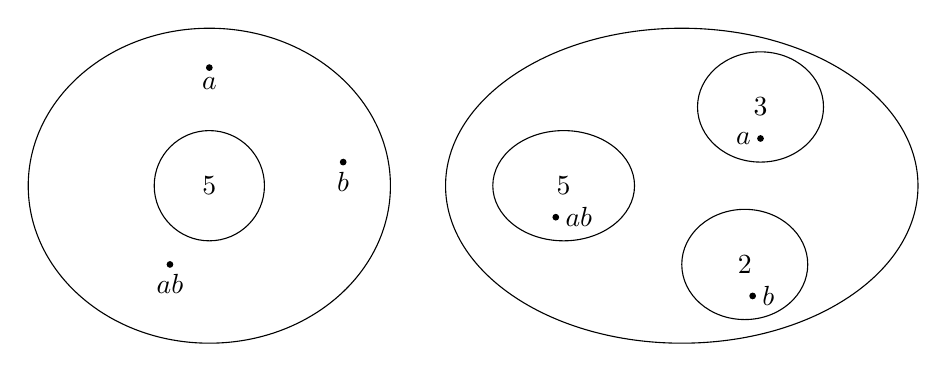
\begin{tikzpicture}
	\filldraw (0,1.5) circle (1pt) node[below] {$a$};
	\filldraw (-.5,-1) circle (1pt) node[below] {$ab$};
	\filldraw (1.7,.3) circle (1pt) node[below] {$b$};
	\node (z5) at (0,0) {$5\Z$};
	
	\draw (z5) ellipse (.7 and .7);
	\draw (z5) ellipse (2.3 and 2);
	
	\begin{scope}[shift={(6,0)}]
	\filldraw (-1.6,-.4) circle (1pt) node[right] {$ab$};
	\filldraw (1,.6) circle (1pt) node[left] {$a$};
	\filldraw (.9,-1.4) circle (1pt) node[right] {$b$};
	\node (z6) at (-1.5,0) {$5\Z$};
	\node (z3) at (1, 1) {$3\Z$};
	\node (z2) at (.8, -1) {$2\Z$};
	\node (op) at (0,0) {};
	
	\draw (z6) ellipse (.9 and .7);
	\draw (z3) ellipse (.8 and .7);
	\draw (z2) ellipse (.8 and .7);
	\draw (op) ellipse (3 and 2);
	\end{scope}
	\end{tikzpicture}
	\caption{Ejemplo de un ideal primo ($5\Z$) y otro no primo ($6\Z$).}
\end{figure}

\begin{ej}
	En $\Z$ el $\{\0\}$ es un ideal primo. También lo es $5\Z$. Por el contrario $6\Z$ no lo es.\footnote{Vaya que chorprecha que los $p\Z$ con $p$ primo sean ideales primos.}
\end{ej}

%TODO probar
\begin{pro}
	Un anillo $A$ es un \gls{di} $\iff \{\0\}$ es un ideal primo.
\end{pro}

Orlando dio la implicación hacia la derecha de este teorema pero \cite{dor96} da la otra.

\begin{pro}
	Sea $P \subsetneq A$ un ideal propio. Entonces $A/P$ \gls{di} $\iff P$ ideal primo.
\end{pro}

\begin{proof}Ver \cite[p.~201]{dor96}.
\end{proof}



\subsection{Ideales maximales}

\begin{dfn}[Ideal maximal]
	Sea $I \subsetneq A$ un ideal propio. Diremos que $I$ es un ideal maximal $\iff \forall J$
	\begin{align*}
		J \text{ ideal } \land I \subseteq J \subset A \implies J = I \lor J = A
	\end{align*}
\end{dfn}

\begin{pro}
	En el anillo $(\Z, +, \cdot)$ son ideales maximales $p\Z$ con $p$ primo.
\end{pro}

\begin{figure}[h]
	\centering
	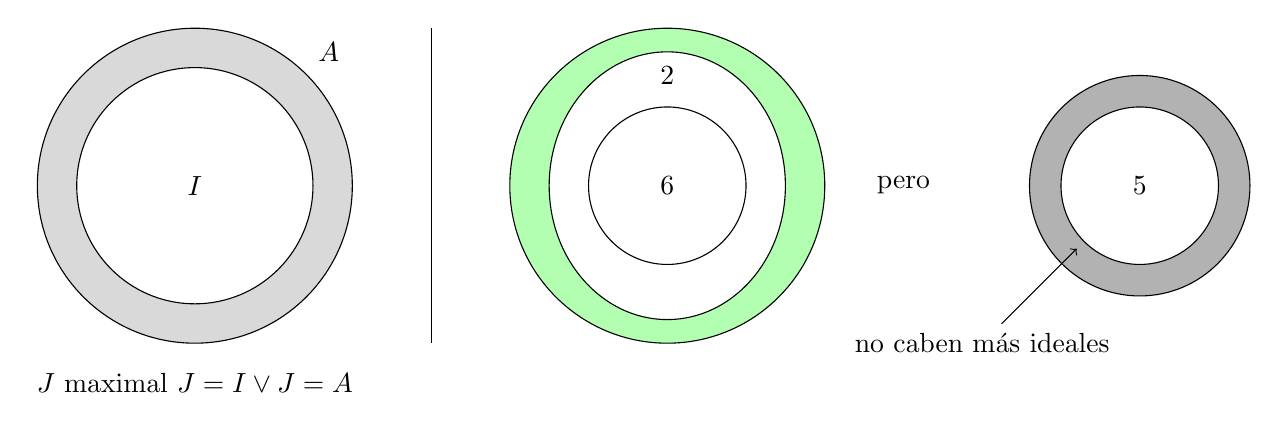
\begin{tikzpicture}
		\draw[black,fill=gray!30] (0,0) ellipse (2 and 2);
		\draw[black,fill=white] (0,0) ellipse (1.5 and 1.5);
		\node (I) at (0,0) {$I$};
		\node (A) at (1.7,1.7) {$A$};
		\node (t) at (0,-2.5) {$J$ maximal $\implies J = I \lor J = A$};
		
		\draw (3,2) -- (3,-2);
		
		\begin{scope}[shift={(6, 0)}]
		\draw[black,fill=green!30] (0,0) ellipse (2 and 2);
		\draw[black,fill=white] (0,0) ellipse (1.5 and 1.7);
		\draw[black,fill=white] (0,0) ellipse (1 and 1);
		\node (6z) at (0,0) {$6\Z$};
		\node (2z) at (0,1.4) {$2\Z$};
		\node (z) at (1.7,1.7) {$\Z$};
		\end{scope}
		
		\node (pero) at (9,0) {pero};
		
		\begin{scope}[shift={(12, 0)}]
		\draw[black,fill=gray!60] (0,0) ellipse (1.4 and 1.4);
		\draw[black,fill=white] (0,0) ellipse (1 and 1);
		\node (5z) at (0,0) {$5\Z$};
		\node (z) at (1.2,1.2) {$\Z$};
		
		\node (nota) at (-2,-2) {no caben más ideales};
		\draw[->] (nota) -- (-0.8, -0.8); 
		\end{scope}
	\end{tikzpicture}
	\caption{Diferencia entre un ideal maximal y uno no maximal. Aquí $6\Z$ no es maximal pero $5\Z$ sí que lo es.}
\end{figure}

\begin{pro}
	\label{pro:maximalcuerpo}
	Sea $M \subsetneq A$ un ideal maximal de $A$. Entonces $A/M$ es un cuerpo.
\end{pro}

\begin{pro}
	\label{pro:maximalimplicaprimo}
	Todo ideal maximal es un ideal primo.
\end{pro}

\begin{proof}
	$M \subsetneq$ un ideal maximal de $A \implies A/M$ cuerpo $\implies A/M$ DI $\implies M$ ideal primo.
\end{proof}

% TODO dar el ejemplo cuando lleguemos al producto directo
El recíproco no es verdad en general. Por ejemplo en $\Z$ el $\{\0\}$ es un ideal primo pero no es maximal porque $\Z/\{\0\} \isom \Z$ no es un cuerpo (contrarrecíproco de la \autoref{pro:maximalcuerpo}).

\subsection{Ideales y el producto directo}

\begin{pro}
	Sean $A, B$ anillos conmutativos con unidad. Sean $I \subset A, J \subset B$ ideales de $A$ y $B$ respectivamente. Entonces $I \times J \subset A \times B$ es un ideal en el producto directo.
\end{pro}

\begin{proof}
	Comprobamos las propiedades de los ideales:
	\begin{enumerate}
		\item $\0 = (0,0) \in I \times J$ porque $\0 \in I \land \0 \in J$
		\item $\forall s = (s_1, s_2), t = (t_1, t_2) \in I \times J$ tenemos que $s + t = (s_1 + t_1, s_2 + t_2) \in I \times J$ pues $s_1, t_1 \in I \implies s_1 + t_1 \in I$ y pasa lo mismo con $s_2$ y $t_2$.
		\item $\forall s = (s_1, s_2) \in I \times J,\ a = (a_1, a_2) \in A \times b$ se tiene que $sa = (s_1 a_1, s_2 a_2) \in I \times J$ pues $s_1a_1 \in I \land s_2 a_2 \in J$. Se tiene lo mismo para el producto por la derecha ya que $A$ y $B$ son conmutativos.
	\end{enumerate}
\end{proof}

%TODO poner un ejemplo con Z/2 \times Z/2




